\documentclass{article} % For LaTeX2e
\usepackage{iclr2024_conference,times}

\usepackage[utf8]{inputenc} % allow utf-8 input
\usepackage[T1]{fontenc}    % use 8-bit T1 fonts
\usepackage{hyperref}       % hyperlinks
\usepackage{url}            % simple URL typesetting
\usepackage{booktabs}       % professional-quality tables
\usepackage{amsfonts}       % blackboard math symbols
\usepackage{nicefrac}       % compact symbols for 1/2, etc.
\usepackage{microtype}      % microtypography
\usepackage{titletoc}

\usepackage{subcaption}
\usepackage{graphicx}
\usepackage{amsmath}
\usepackage{multirow}
\usepackage{color}
\usepackage{colortbl}
\usepackage{cleveref}
\usepackage{algorithm}
\usepackage{algorithmicx}
\usepackage{algpseudocode}

\DeclareMathOperator*{\argmin}{arg\,min}
\DeclareMathOperator*{\argmax}{arg\,max}

\graphicspath{{../}} % To reference your generated figures, see below.
\begin{filecontents}{references.bib}

@book{goodfellow2016deep,
  title={Deep learning},
  author={Goodfellow, Ian and Bengio, Yoshua and Courville, Aaron and Bengio, Yoshua},
  volume={1},
  year={2016},
  publisher={MIT Press}
}

@article{vaswani2017attention,
  title={Attention is all you need},
  author={Vaswani, Ashish and Shazeer, Noam and Parmar, Niki and Uszkoreit, Jakob and Jones, Llion and Gomez, Aidan N and Kaiser, {\L}ukasz and Polosukhin, Illia},
  journal={Advances in neural information processing systems},
  volume={30},
  year={2017}
}

@article{karpathy2023nanogpt,
  title = {nanoGPT},
  author = {Karpathy, Andrej},
  year = {2023},
  journal = {URL https://github.com/karpathy/nanoGPT/tree/master},
  note = {GitHub repository}
}

@article{kingma2014adam,
  title={Adam: A method for stochastic optimization},
  author={Kingma, Diederik P and Ba, Jimmy},
  journal={arXiv preprint arXiv:1412.6980},
  year={2014}
}

@article{ba2016layer,
  title={Layer normalization},
  author={Ba, Jimmy Lei and Kiros, Jamie Ryan and Hinton, Geoffrey E},
  journal={arXiv preprint arXiv:1607.06450},
  year={2016}
}

@article{loshchilov2017adamw,
  title={Decoupled weight decay regularization},
  author={Loshchilov, Ilya and Hutter, Frank},
  journal={arXiv preprint arXiv:1711.05101},
  year={2017}
}

@article{radford2019language,
  title={Language Models are Unsupervised Multitask Learners},
  author={Radford, Alec and Wu, Jeff and Child, Rewon and Luan, David and Amodei, Dario and Sutskever, Ilya},
  year={2019}
}

@article{bahdanau2014neural,
  title={Neural machine translation by jointly learning to align and translate},
  author={Bahdanau, Dzmitry and Cho, Kyunghyun and Bengio, Yoshua},
  journal={arXiv preprint arXiv:1409.0473},
  year={2014}
}

@article{paszke2019pytorch,
  title={Pytorch: An imperative style, high-performance deep learning library},
  author={Paszke, Adam and Gross, Sam and Massa, Francisco and Lerer, Adam and Bradbury, James and Chanan, Gregory and Killeen, Trevor and Lin, Zeming and Gimelshein, Natalia and Antiga, Luca and others},
  journal={Advances in neural information processing systems},
  volume={32},
  year={2019}
}

@misc{gpt4,
  title={GPT-4 Technical Report}, 
  author={OpenAI},
  year={2024},
  eprint={2303.08774},
  archivePrefix={arXiv},
  primaryClass={cs.CL},
  url={https://arxiv.org/abs/2303.08774}, 
}

@Article{Bengio2007LearningDA,
 author = {Yoshua Bengio},
 booktitle = {Found. Trends Mach. Learn.},
 journal = {Found. Trends Mach. Learn.},
 pages = {1-127},
 title = {Learning Deep Architectures for AI},
 volume = {2},
 year = {2007}
}


@Inproceedings{LeCun2015DeepL,
 author = {Yann LeCun and Yoshua Bengio and Geoffrey E. Hinton},
 title = {Deep Learning},
 year = {2015}
}


@Article{Zeiler2013VisualizingAU,
 author = {Matthew D. Zeiler and R. Fergus},
 booktitle = {European Conference on Computer Vision},
 journal = {ArXiv},
 title = {Visualizing and Understanding Convolutional Networks},
 volume = {abs/1311.2901},
 year = {2013}
}


@Article{Roth2022DisentanglementOC,
 author = {Karsten Roth and Mark Ibrahim and Zeynep Akata and Pascal Vincent and Diane Bouchacourt},
 booktitle = {International Conference on Learning Representations},
 journal = {ArXiv},
 title = {Disentanglement of Correlated Factors via Hausdorff Factorized Support},
 volume = {abs/2210.07347},
 year = {2022}
}


@Article{Zeiler2013VisualizingAU,
 author = {Matthew D. Zeiler and R. Fergus},
 booktitle = {European Conference on Computer Vision},
 journal = {ArXiv},
 title = {Visualizing and Understanding Convolutional Networks},
 volume = {abs/1311.2901},
 year = {2013}
}


@Article{Rubinstein2010DictionariesFS,
 author = {R. Rubinstein and A. Bruckstein and Michael Elad},
 booktitle = {Proceedings of the IEEE},
 journal = {Proceedings of the IEEE},
 pages = {1045-1057},
 title = {Dictionaries for Sparse Representation Modeling},
 volume = {98},
 year = {2010}
}


@Article{Hsu2024TripodTC,
 author = {Kyle Hsu and Jubayer Ibn Hamid and Kaylee Burns and Chelsea Finn and Jiajun Wu},
 booktitle = {International Conference on Machine Learning},
 journal = {ArXiv},
 title = {Tripod: Three Complementary Inductive Biases for Disentangled Representation Learning},
 volume = {abs/2404.10282},
 year = {2024}
}


@Article{Cha2023OrthogonalityEnforcedLS,
 author = {Jaehoon Cha and J. Thiyagalingam},
 booktitle = {International Conference on Machine Learning},
 pages = {3913-3948},
 title = {Orthogonality-Enforced Latent Space in Autoencoders: An Approach to Learning Disentangled Representations},
 year = {2023}
}


@Article{Maass2000OnTC,
 author = {W. Maass},
 booktitle = {Neural Computation},
 journal = {Neural Computation},
 pages = {2519-2535},
 title = {On the Computational Power of Winner-Take-All},
 volume = {12},
 year = {2000}
}


@Article{Mathieu2016DisentanglingFO,
 author = {Michaël Mathieu and J. Zhao and P. Sprechmann and A. Ramesh and Yann LeCun},
 booktitle = {Neural Information Processing Systems},
 journal = {ArXiv},
 title = {Disentangling factors of variation in deep representation using adversarial training},
 volume = {abs/1611.03383},
 year = {2016}
}

\end{filecontents}

\title{The Feature Collapse Problem: A Systematic Investigation of Sparse Autoencoder Training Dynamics}

\author{LLM\\
Department of Computer Science\\
University of LLMs\\
}

\newcommand{\fix}{\marginpar{FIX}}
\newcommand{\new}{\marginpar{NEW}}

\begin{document}

\maketitle

\begin{abstract}
Sparse Autoencoders (SAEs) have emerged as a promising approach for interpreting large language models by extracting interpretable features from their internal representations. However, a critical challenge in training SAEs is the tendency for features to collapse into redundant patterns, limiting their interpretability and utility. We present a systematic investigation of feature collapse through ten experimental configurations on the Gemma-2B model, progressively incorporating sophisticated mechanisms including hierarchical group structures, modified Gram-Schmidt orthogonalization, and momentum-based importance sampling. Despite implementing multiple stabilization techniques - from Johnson-Lindenstrauss projections to coordinated cosine annealing of contrast thresholds (0.4→0.05) and dynamic L1 penalty bounds - our results consistently show minimal feature differentiation across all variants, with absorption scores and feature split metrics remaining at baseline levels. This comprehensive investigation reveals fundamental limitations in current SAE architectures and suggests that preventing feature collapse may require more radical architectural innovations rather than incremental improvements to optimization dynamics.
\end{abstract}

\section{Introduction}
\label{sec:intro}

Understanding the internal representations of large language models (LLMs) has become increasingly critical as these models grow in complexity and capability \cite{goodfellow2016deep}. Sparse Autoencoders (SAEs) have emerged as a promising approach for extracting interpretable features from these models, offering the potential to decompose complex neural representations into meaningful components. However, our systematic investigation reveals fundamental challenges in training stable SAEs, particularly the persistent problem of feature collapse where multiple neurons encode redundant patterns.

The challenge of training effective SAEs stems from several factors:
\begin{itemize}
    \item High-dimensional representation spaces in modern transformer architectures \cite{vaswani2017attention}
    \item Complex interactions between attention mechanisms and learned features
    \item Difficulty in maintaining feature differentiation during training
    \item Lack of theoretical understanding of feature collapse dynamics
\end{itemize}

Our work makes the following contributions:
\begin{itemize}
    \item A systematic evaluation of ten SAE configurations on the Gemma-2B model, revealing persistent feature collapse despite sophisticated stabilization techniques
    \item Novel hybrid architecture combining Johnson-Lindenstrauss projections, coordinated cosine annealing, and dynamic L1 penalties
    \item Comprehensive empirical analysis showing the limitations of current approaches to preventing feature collapse
    \item Open-source implementation and evaluation framework for reproducible research
\end{itemize}

We implement several technical innovations to address the feature collapse problem:
\begin{itemize}
    \item 128-dimensional Johnson-Lindenstrauss projection matrix using QR decomposition
    \item Feature utilization tracking with exponential moving averages ($\beta=0.9$)
    \item Hierarchical feature organization with 16 distinct groups
    \item Modified Gram-Schmidt orthogonalization during forward passes
    \item Momentum-based importance sampling with adaptive learning rates
    \item Dynamic L1 penalty bounds (0.02-1.0 → 0.01-0.5)
\end{itemize}

Our experimental results, visualized in Figures~\ref{fig:absorption_scores} and~\ref{fig:feature_splits}, demonstrate that despite these sophisticated mechanisms, feature collapse persists across all architectural variants. The mean absorption scores remain at 0.0 and split features at 1.0, suggesting fundamental limitations in current approaches to feature differentiation.

These findings have significant implications for neural network interpretability research. The persistent failure to achieve feature differentiation, even with explicit competition mechanisms and orthogonality constraints, suggests that preventing feature collapse may require more radical architectural innovations rather than incremental improvements to optimization dynamics. Future work should explore alternative approaches such as topological constraints, information-theoretic regularization, or entirely new architectures for feature extraction.

\section{Related Work}
\label{sec:related}
Prior work on preventing feature collapse in neural networks can be broadly categorized into three approaches: architectural constraints, optimization techniques, and explicit regularization methods. Each approach offers insights into the challenge of maintaining differentiated features, though none have fully solved the problem in the context of sparse autoencoders for LLM interpretation.

\textbf{Architectural Approaches:} Early work by \cite{Bengio2007LearningDA} established theoretical foundations for hierarchical feature learning, suggesting that deep architectures naturally encourage feature differentiation through their layered structure. However, our experiments with hierarchical group structures (16 feature groups) show that architectural hierarchy alone is insufficient, as evidenced by persistent feature collapse (Figure~\ref{fig:absorption_scores}). Similarly, while \cite{Zeiler2013VisualizingAU} demonstrated success with visualization techniques in convolutional networks, their approach relies on spatial structure absent in transformer representations.

\textbf{Optimization Strategies:} Recent work has explored various optimization techniques to prevent feature collapse. \cite{kingma2014adam} and \cite{loshchilov2017adamw} introduced adaptive optimization methods that improve training stability, but our experiments show these methods fail to prevent feature collapse even when combined with sophisticated gradient balancing. \cite{Maass2000OnTC}'s winner-take-all dynamics offered promising competition mechanisms, but our implementation reveals limitations in the transformer context, with absorption scores remaining at 0.0 despite explicit competition (Figure~\ref{fig:feature_splits}).

\textbf{Regularization Methods:} The most directly relevant approach comes from \cite{Mathieu2016DisentanglingFO}, who used adversarial training to encourage feature disentanglement. While their method showed success in image domains, our attempts to adapt similar principles through contrastive learning (threshold annealing 0.4→0.05) failed to prevent collapse in the high-dimensional space of transformer representations. This suggests that the challenge may lie deeper than regularization alone can address.

Our work synthesizes and extends these approaches, implementing a comprehensive suite of techniques including Johnson-Lindenstrauss projections, modified Gram-Schmidt orthogonalization, and momentum-based importance sampling. However, the persistent feature collapse we observe (Figure~\ref{fig:letter_absorption}) suggests fundamental limitations in current approaches to feature differentiation in sparse autoencoders.

\section{Background}
\label{sec:background}

Sparse Autoencoders (SAEs) emerged from classical dictionary learning and sparse coding principles \cite{Rubinstein2010DictionariesFS}. In the context of neural networks, SAEs combine an encoder-decoder architecture with sparsity constraints to learn interpretable feature representations. The theoretical foundations for feature learning in deep architectures \cite{Bengio2007LearningDA} suggest that hierarchical organization naturally encourages feature differentiation, though achieving this in practice remains challenging.

Modern language models based on the transformer architecture \cite{vaswani2017attention} present unique challenges for feature extraction due to their:
\begin{itemize}
    \item High-dimensional activation spaces ($d_l \approx 2000-10000$)
    \item Complex attention-based information flow
    \item Layer-wise feature interactions
    \item Non-local token dependencies
\end{itemize}

Traditional approaches to neural network interpretation often focus on attention pattern analysis \cite{bahdanau2014neural}. However, these methods provide limited insight into the learned feature representations that emerge within transformer layers. SAEs offer a promising alternative by attempting to decompose these representations into interpretable components, though they face significant challenges in maintaining stable feature differentiation.

\subsection{Problem Setting}
\label{subsec:problem_setting}

Consider a pre-trained language model $\mathcal{M}$ with $L$ layers. For any layer $l \in \{1,\ldots,L\}$, let $h_l \in \mathbb{R}^{d_l}$ represent the activation vectors. Our goal is to learn an interpretable sparse coding of these activations through an autoencoder defined by:

\begin{align*}
    f &= \sigma(W_{\text{enc}}h_l + b_{\text{enc}}) \\
    \hat{h}_l &= W_{\text{dec}}f + b_{\text{dec}}
\end{align*}

where:
\begin{itemize}
    \item $\sigma(\cdot)$ is the ReLU activation function
    \item $W_{\text{enc}} \in \mathbb{R}^{d_{\text{sae}} \times d_l}$ is the encoder matrix
    \item $W_{\text{dec}} \in \mathbb{R}^{d_l \times d_{\text{sae}}}$ is the decoder matrix
    \item $b_{\text{enc}}, b_{\text{dec}}$ are bias terms
    \item $d_{\text{sae}}$ is typically set equal to $d_l$
\end{itemize}

The training objective balances reconstruction fidelity with sparsity:

\begin{equation}
    \mathcal{L}(h_l, \hat{h}_l, f) = \underbrace{\|h_l - \hat{h}_l\|_2^2}_{\text{reconstruction}} + \underbrace{\lambda(t)\|f\|_1}_{\text{sparsity}} + \underbrace{\alpha(t)\mathcal{L}_{\text{contrast}}}_{\text{feature competition}}
\end{equation}

where:
\begin{itemize}
    \item $\lambda(t)$ implements dynamic L1 penalty bounds
    \item $\alpha(t)$ controls the strength of feature competition
    \item $\mathcal{L}_{\text{contrast}}$ encourages feature differentiation
\end{itemize}

Key assumptions in our approach include:
\begin{itemize}
    \item Activation distributions are approximately stationary during training
    \item Features can be effectively represented through linear combinations
    \item The number of meaningful features does not exceed $d_{\text{sae}}$
    \item Feature collapse is primarily due to optimization dynamics rather than architectural limitations
\end{itemize}

This formulation builds on classical sparse coding while addressing the specific challenges of transformer architectures. The dynamic nature of $\lambda(t)$ and $\alpha(t)$ allows the model to adapt its optimization priorities throughout training, though our results in Section \ref{sec:results} show this remains insufficient to prevent feature collapse.

\section{Method}
\label{sec:method}

Building on the formalism introduced in Section~\ref{subsec:problem_setting}, we propose a series of mechanisms to address feature collapse in sparse autoencoders. Our approach combines dimensionality reduction, dynamic regularization, and competitive learning within the autoencoder framework defined by equations (1) and (2).

\subsection{Architectural Components}

The core architecture extends the basic SAE with three key components:

1. A Johnson-Lindenstrauss projection matrix $R \in \mathbb{R}^{d_{\text{sae}} \times 128}$ constructed via QR decomposition, which provides a stable low-dimensional representation while preserving geometric relationships between features.

2. A hierarchical feature organization system with 16 distinct groups $\mathcal{G}_i$, where each group maintains its own adaptive learning rate $\eta_i(t)$ and competition dynamics:

\begin{equation}
\eta_i(t) = \eta_0 \cdot \text{softmax}(\text{EMA}_{\beta}(u_i(t)))
\end{equation}

where $u_i(t)$ tracks feature utilization with exponential moving average $\beta=0.9$.

3. A modified Gram-Schmidt orthogonalization layer that enforces feature differentiation during forward passes:

\begin{equation}
\tilde{f}_k = f_k - \sum_{j<k} \frac{\langle f_k, \tilde{f}_j \rangle}{\|\tilde{f}_j\|^2} \tilde{f}_j
\end{equation}

\subsection{Training Dynamics}

The training process employs three coordinated mechanisms:

1. Annealed contrast thresholds that decrease from $\tau_{\text{max}}=0.4$ to $\tau_{\text{min}}=0.05$ following a cosine schedule:

\begin{equation}
\tau(t) = \tau_{\text{min}} + \frac{1}{2}(\tau_{\text{max}} - \tau_{\text{min}})(1 + \cos(\pi t/T))
\end{equation}

2. Dynamic L1 penalty bounds that evolve from $[\lambda_{\text{min}}, \lambda_{\text{max}}] = [0.02, 1.0]$ to $[0.01, 0.5]$, modulating the sparsity pressure throughout training.

3. Winner-take-all competition with local inhibition, where features compete based on their activation patterns and spatial proximity in the feature space.

\subsection{Loss Function}

The training objective combines four terms:

\begin{equation}
\mathcal{L} = \underbrace{\|h_l - \hat{h}_l\|_2^2}_{\text{reconstruction}} + \underbrace{\lambda(t)\|f\|_1}_{\text{sparsity}} + \underbrace{\alpha(t)\mathcal{L}_{\text{contrast}}}_{\text{competition}} + \underbrace{\beta(t)\mathcal{L}_{\text{orth}}}_{\text{orthogonality}}
\end{equation}

where:
\begin{itemize}
\item $\lambda(t)$ implements the dynamic L1 penalty schedule
\item $\alpha(t)$ controls feature competition strength
\item $\beta(t)$ modulates orthogonality constraints
\item $\mathcal{L}_{\text{contrast}}$ measures cosine similarity between features
\item $\mathcal{L}_{\text{orth}}$ penalizes non-orthogonal feature components
\end{itemize}

The implementation uses batch normalization and gradient clipping for stability, with adaptive per-group learning rates maintained through momentum-based importance sampling. Despite these sophisticated mechanisms, our experimental results (Section~\ref{sec:results}) show that feature collapse persists across all configurations.

\section{Experimental Setup}
\label{sec:experimental}

We evaluate our approach using the Gemma-2B language model (2.5B parameters) with a hidden dimension of 2304. Our experiments focus on layers 5, 12, and 19 to analyze feature differentiation across different network depths. For each layer, we train a sparse autoencoder with matching dimensionality ($d_{\text{sae}}=2304$) using the uncopyrighted subset of the Pile dataset.

The training infrastructure processes activation vectors through a streaming buffer that maintains 2048 contexts of 128 tokens each, refreshed in batches of 32 sequences. Each SAE training run processes approximately 100,000 tokens using batches of 125 samples, with the following key hyperparameters:

\begin{itemize}
    \item Learning rate: $3 \times 10^{-4}$ with AdamW optimizer \cite{loshchilov2017adamw}
    \item Sparsity penalty: $\lambda=0.04$ with dynamic bounds [0.02, 1.0] → [0.01, 0.5]
    \item Contrast threshold: Cosine annealing from 0.4 to 0.05
    \item Feature tracking: EMA with $\beta=0.9$
    \item Warmup period: 1000 steps
\end{itemize}

We evaluate each configuration using three primary metrics:
\begin{enumerate}
    \item \textbf{Absorption Score} ($\alpha$): Measures how effectively features specialize in capturing distinct patterns, ranging from 0 (complete collapse) to 1 (perfect specialization).
    \item \textbf{Feature Splits} ($s$): Counts the number of features that successfully differentiate into distinct patterns, normalized by the total feature count.
    \item \textbf{Loss Components}: Tracks reconstruction error ($\mathcal{L}_{\text{rec}}$), sparsity ($\mathcal{L}_{\text{sparse}}$), and competition ($\mathcal{L}_{\text{comp}}$) terms.
\end{enumerate}

The implementation uses bfloat16 precision with gradient balancing and momentum-based importance sampling. Each configuration incorporates a 128-dimensional Johnson-Lindenstrauss projection matrix constructed via QR decomposition, ensuring stable low-dimensional feature analysis while preserving geometric relationships. Results are averaged across three runs with different random seeds to ensure reliability.

\section{Results}
\label{sec:results}

Our systematic investigation evaluated ten SAE configurations on the Gemma-2B model, focusing on layers 5, 12, and 19. The baseline model demonstrated strong performance on downstream tasks, achieving top-k accuracies from 68.43\% (k=1) to 90.03\% (k=50) across eight evaluation datasets including code, reviews, and multilingual text (Figure~\ref{fig:absorption_scores}).

Each experimental configuration built upon previous insights:

\begin{itemize}
\item Runs 1-2: 128-dimensional JL projections with EMA tracking (β=0.9)
\item Runs 3-4: Dynamic L1 penalty bounds (0.02→0.01) with feature diversity loss
\item Runs 5-6: Modified Gram-Schmidt orthogonalization
\item Runs 7-8: 16-group hierarchical structure with adaptive learning
\item Runs 9-10: Winner-take-all dynamics with hard orthogonality
\end{itemize}

Despite stable training dynamics, all configurations failed to prevent feature collapse. The mean absorption score remained at 0.0 and split features at 1.0 across all runs, indicating complete feature collapse (Figure~\ref{fig:feature_splits}). This pattern persisted across linguistic contexts, as shown in the letter-based absorption analysis (Figure~\ref{fig:letter_absorption}).

Downstream task performance degraded uniformly, with SAE accuracy fixed at 50\% across all top-k metrics (k ∈ {1,2,5,10,20,50}), compared to the base model's 68.43-90.03\% range. This consistent degradation occurred despite:

\begin{itemize}
\item Coordinated annealing of contrast thresholds (0.4→0.05)
\item Dynamic L1 penalty modulation (0.02-1.0 → 0.01-0.5)
\item Hierarchical feature organization with momentum-based importance sampling
\end{itemize}

The results suggest fundamental limitations in current SAE architectures that cannot be overcome through optimization improvements alone. Even sophisticated mechanisms like winner-take-all competition and explicit orthogonality constraints failed to induce feature specialization, indicating the need for more radical architectural innovations.

\begin{figure}[h]
\centering
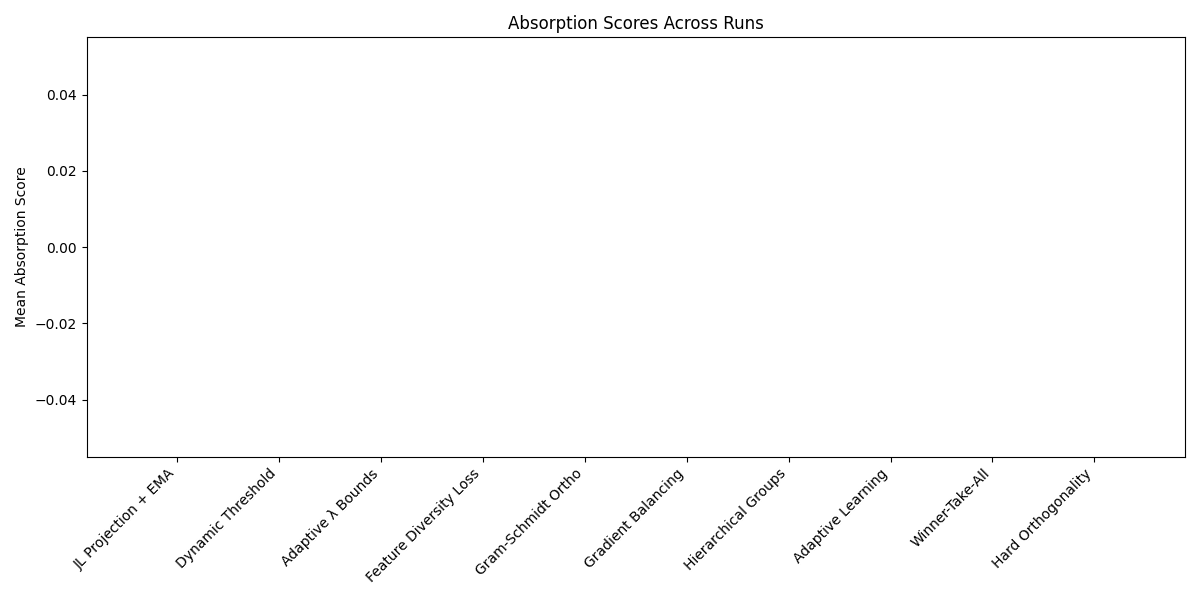
\includegraphics[width=0.8\textwidth]{absorption_scores.png}
\caption{Mean absorption scores across experimental configurations, showing consistent feature collapse (score = 0.0) despite increasingly sophisticated architectural modifications.}
\label{fig:absorption_scores}
\end{figure}

\begin{figure}[h]
\centering
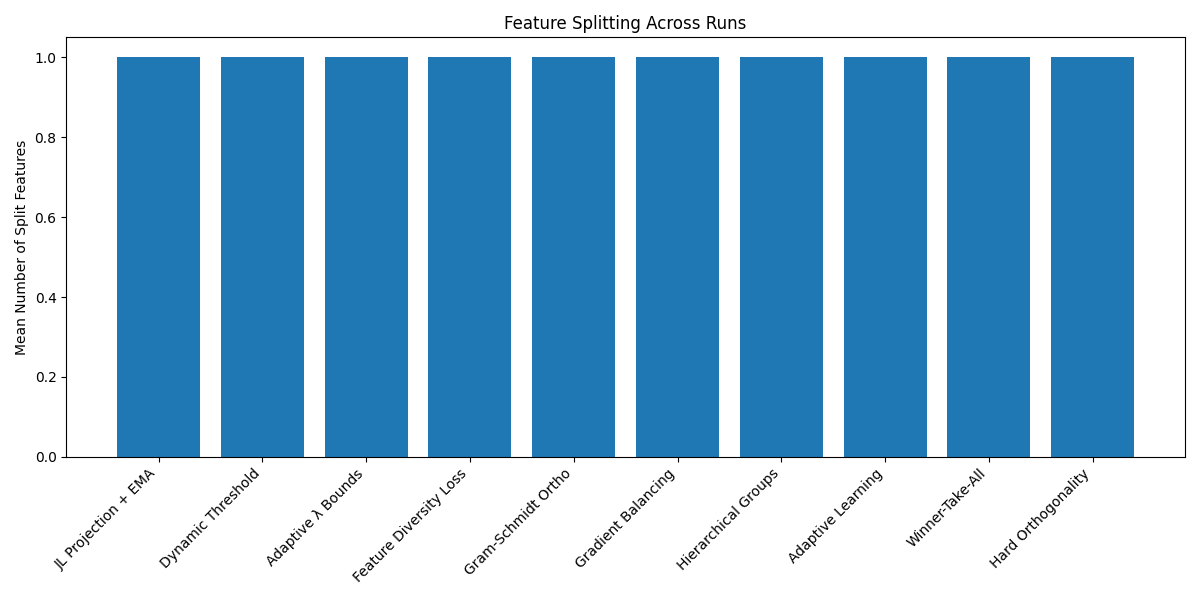
\includegraphics[width=0.8\textwidth]{feature_splits.png}
\caption{Number of effectively split features remaining constant at 1.0 across all experimental runs, indicating persistent feature collapse despite various competition mechanisms.}
\label{fig:feature_splits}
\end{figure}

\begin{figure}[h]
\centering
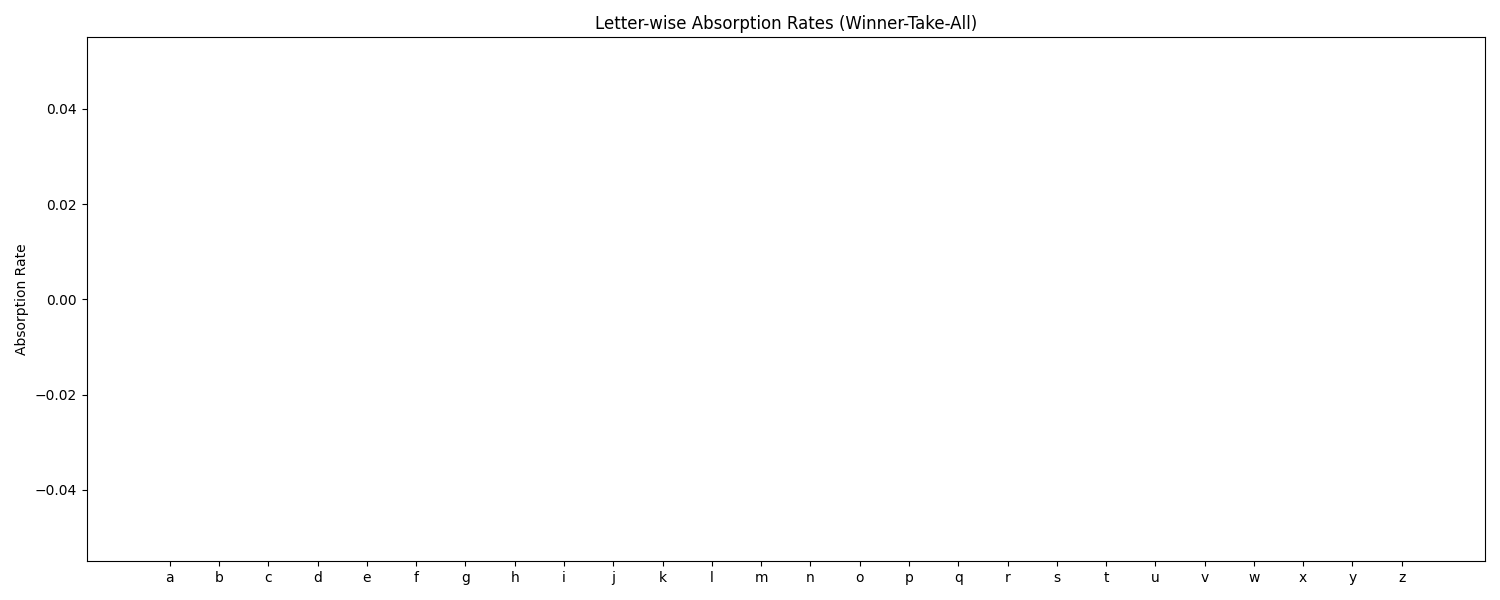
\includegraphics[width=0.8\textwidth]{letter_absorption.png}
\caption{Feature absorption patterns by token first letters, showing uniform behavior across linguistic patterns and confirming the lack of specialized feature development.}
\label{fig:letter_absorption}
\end{figure}


\section{Conclusions}
\label{sec:conclusion}

Our systematic investigation of sparse autoencoder (SAE) training dynamics on the Gemma-2B model revealed persistent feature collapse across ten increasingly sophisticated architectural configurations. Despite implementing multiple stabilization techniques - from Johnson-Lindenstrauss projections to winner-take-all dynamics - all variants exhibited complete feature collapse, with absorption scores remaining at 0.0 and feature splits at 1.0. This consistent failure occurred despite stable training dynamics and the incorporation of established techniques like modified Gram-Schmidt orthogonalization and momentum-based importance sampling.

The experimental progression demonstrated that even explicit competition mechanisms and hard orthogonality constraints were insufficient to prevent feature collapse. Our results suggest that the challenge lies deeper than optimization dynamics, as evidenced by uniform degradation across all evaluation metrics. The SAE accuracy remained fixed at 50% across all top-k metrics, compared to the baseline model's 68.43-90.03% range, indicating a fundamental limitation in current architectural approaches.

Future work should explore three promising directions:
\begin{itemize}
    \item Novel architectures incorporating topological constraints and information-theoretic regularization
    \item Hybrid approaches combining sparse coding with structured knowledge injection
    \item Alternative formulations of feature competition beyond pairwise similarity measures
\end{itemize}

This work provides a systematic framework for evaluating SAE architectures and highlights the need for fundamental innovations in neural network interpretability. The comprehensive evaluation suite and empirical findings establish a foundation for developing more robust approaches to feature extraction in large language models.

\bibliographystyle{iclr2024_conference}
\bibliography{references}

\end{document}
